\documentclass{beamer}

% Choose a theme (Madrid is a clean, simple option)
\usetheme{Madrid}

% Title and author information
\title[Custom GPU Parser vs cuDF CSV Parser]{Custom GPU Parser vs cuDF CSV Parser \\ and cuDF Parquet vs CPU Methods}
\author{Tarun Sreepada ID: m5281045}
\institute{University of Aizu}
\date{\today}

% Additional packages (if needed)
\usepackage{graphicx}   % For including images
\usepackage{booktabs}   % For nicer tables
\usepackage{hyperref}   % For clickable links
\usepackage{subcaption} % For subfigures
\usepackage{verbatim}
\usepackage{listings}


\begin{document}

% Title Slide
\begin{frame}
  \titlepage
  % \author{Tarun Sreepada}
\end{frame}

% Table of contents
\begin{frame}{Outline}
  \tableofcontents
\end{frame}

% Introduction Slide
\section{Introduction}
\begin{frame}[fragile]{Introduction}
  \begin{itemize}
    \item \textbf{CSV Files:} A file format for storing tabular data in plain text. Encodings can vary, and line sizes can be inconsistent.
    \begin{lstlisting}[caption={CSV file}]
    1,2,3,4,5
    6,7,8,9,10
    11,12,13,14,15
    \end{lstlisting}
    \item \textbf{Encoding Table:} A mapping of bits to characters, such as ASCII or UTF-8.
    % \item In this work, we compare the performance of custom GPU parsers and cuDF CSV parsers for handling CSV files with varying line sizes, with a file containing 32-bit integers encoded in UTF-8, in a comma-separated format.
    % \item Comparison of different approaches:
    %   \begin{itemize}
    %     \item \textbf{Custom GPU Parser}: A tailor-made GPU solution to handle varying line sizes in CSVs.
    %     \item \textbf{cuDF CSV Parser}: A component of the RAPIDS cuDF library that leverages GPU acceleration. Cannot deal with varying line sizes in CSVs.
    %     \item \textbf{cuDF Parquet}: A GPU-accelerated Parquet parser compared with traditional CPU methods.
    %     \item \textbf{CPU Methods}: Traditional CPU-based methods for parsing CSV.
    %   \end{itemize}
    % \item Objective: To analyze performance differences, throughput, and potential trade-offs.
  \end{itemize}

  \begin{figure}
    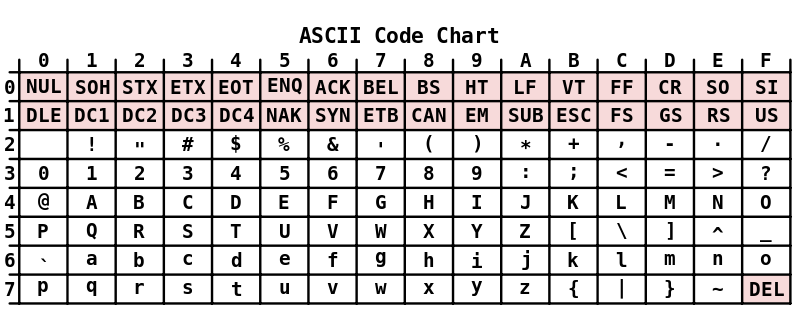
\includegraphics[width=0.6\textwidth]{image copy.png}
    \caption{Encoding Table}
  \end{figure}
\end{frame}

% % Background Slide
% \section{Background}
% \begin{frame}{Background}
%   \begin{itemize}
%     \item \textbf{GPU Acceleration:} Utilizes parallel processing capabilities of GPUs to speed up data parsing and processing.
%     \item \textbf{cuDF Library:} Part of the RAPIDS suite, it provides DataFrame-like operations on GPUs.
%     \item \textbf{CSV and Parquet Formats:}
%       \begin{itemize}
%         \item \textbf{CSV:} A simple, row-based text format.
%         \item \textbf{Parquet:} A columnar storage file format that allows for efficient compression and encoding schemes.
%       \end{itemize}
%     \item \textbf{CPU Methods:} Utilizing multiple threads to split CSV into chunks and parse it.
%   \end{itemize}
% \end{frame}


% Custom GPU Parser Slide
\section{Custom GPU Parser}
\begin{frame}{Custom GPU Parser Approach}
  \begin{itemize}
    \item \textbf{File Loading:}  
      \begin{itemize}
        \item Load the entire CSV file into memory.
      \end{itemize}
    \item \textbf{Transaction Counting:}
      \begin{itemize}
        \item Count the number of newline characters to determine the total number of transactions.
      \end{itemize}
    \item \textbf{Line Boundary Detection:}
      \begin{itemize}
        \item Identify the exact positions of all newline characters to know where each record ends.
      \end{itemize}
    \item \textbf{Item Counting and Memory Allocation:}
      \begin{itemize}
        \item For each newline, count the number of CSV items.
        \item Create a new memory area dedicated for the conversion of UTF-8 encoded integers to unsigned integers.
      \end{itemize}
    \item \textbf{Parallel Parsing:}
      \begin{itemize}
        \item Launch one GPU thread per CSV line (transaction) to parse and convert the data into the newly allocated area.
      \end{itemize}
  \end{itemize}
  % \begin{itemize}
  %   \item \textbf{Downsides}
  %   \item \begin{itemize}
  %     \item \textbf{Memory Utilization:} Requires a copy of the entire file in memory.
  %     \item \textbf{Line Size Limitation:} Limited by the available GPU memory. 
  % \end{itemize}

\end{frame}

\begin{frame}{GPU Read Illustrated}
  \begin{figure}
    \centering
    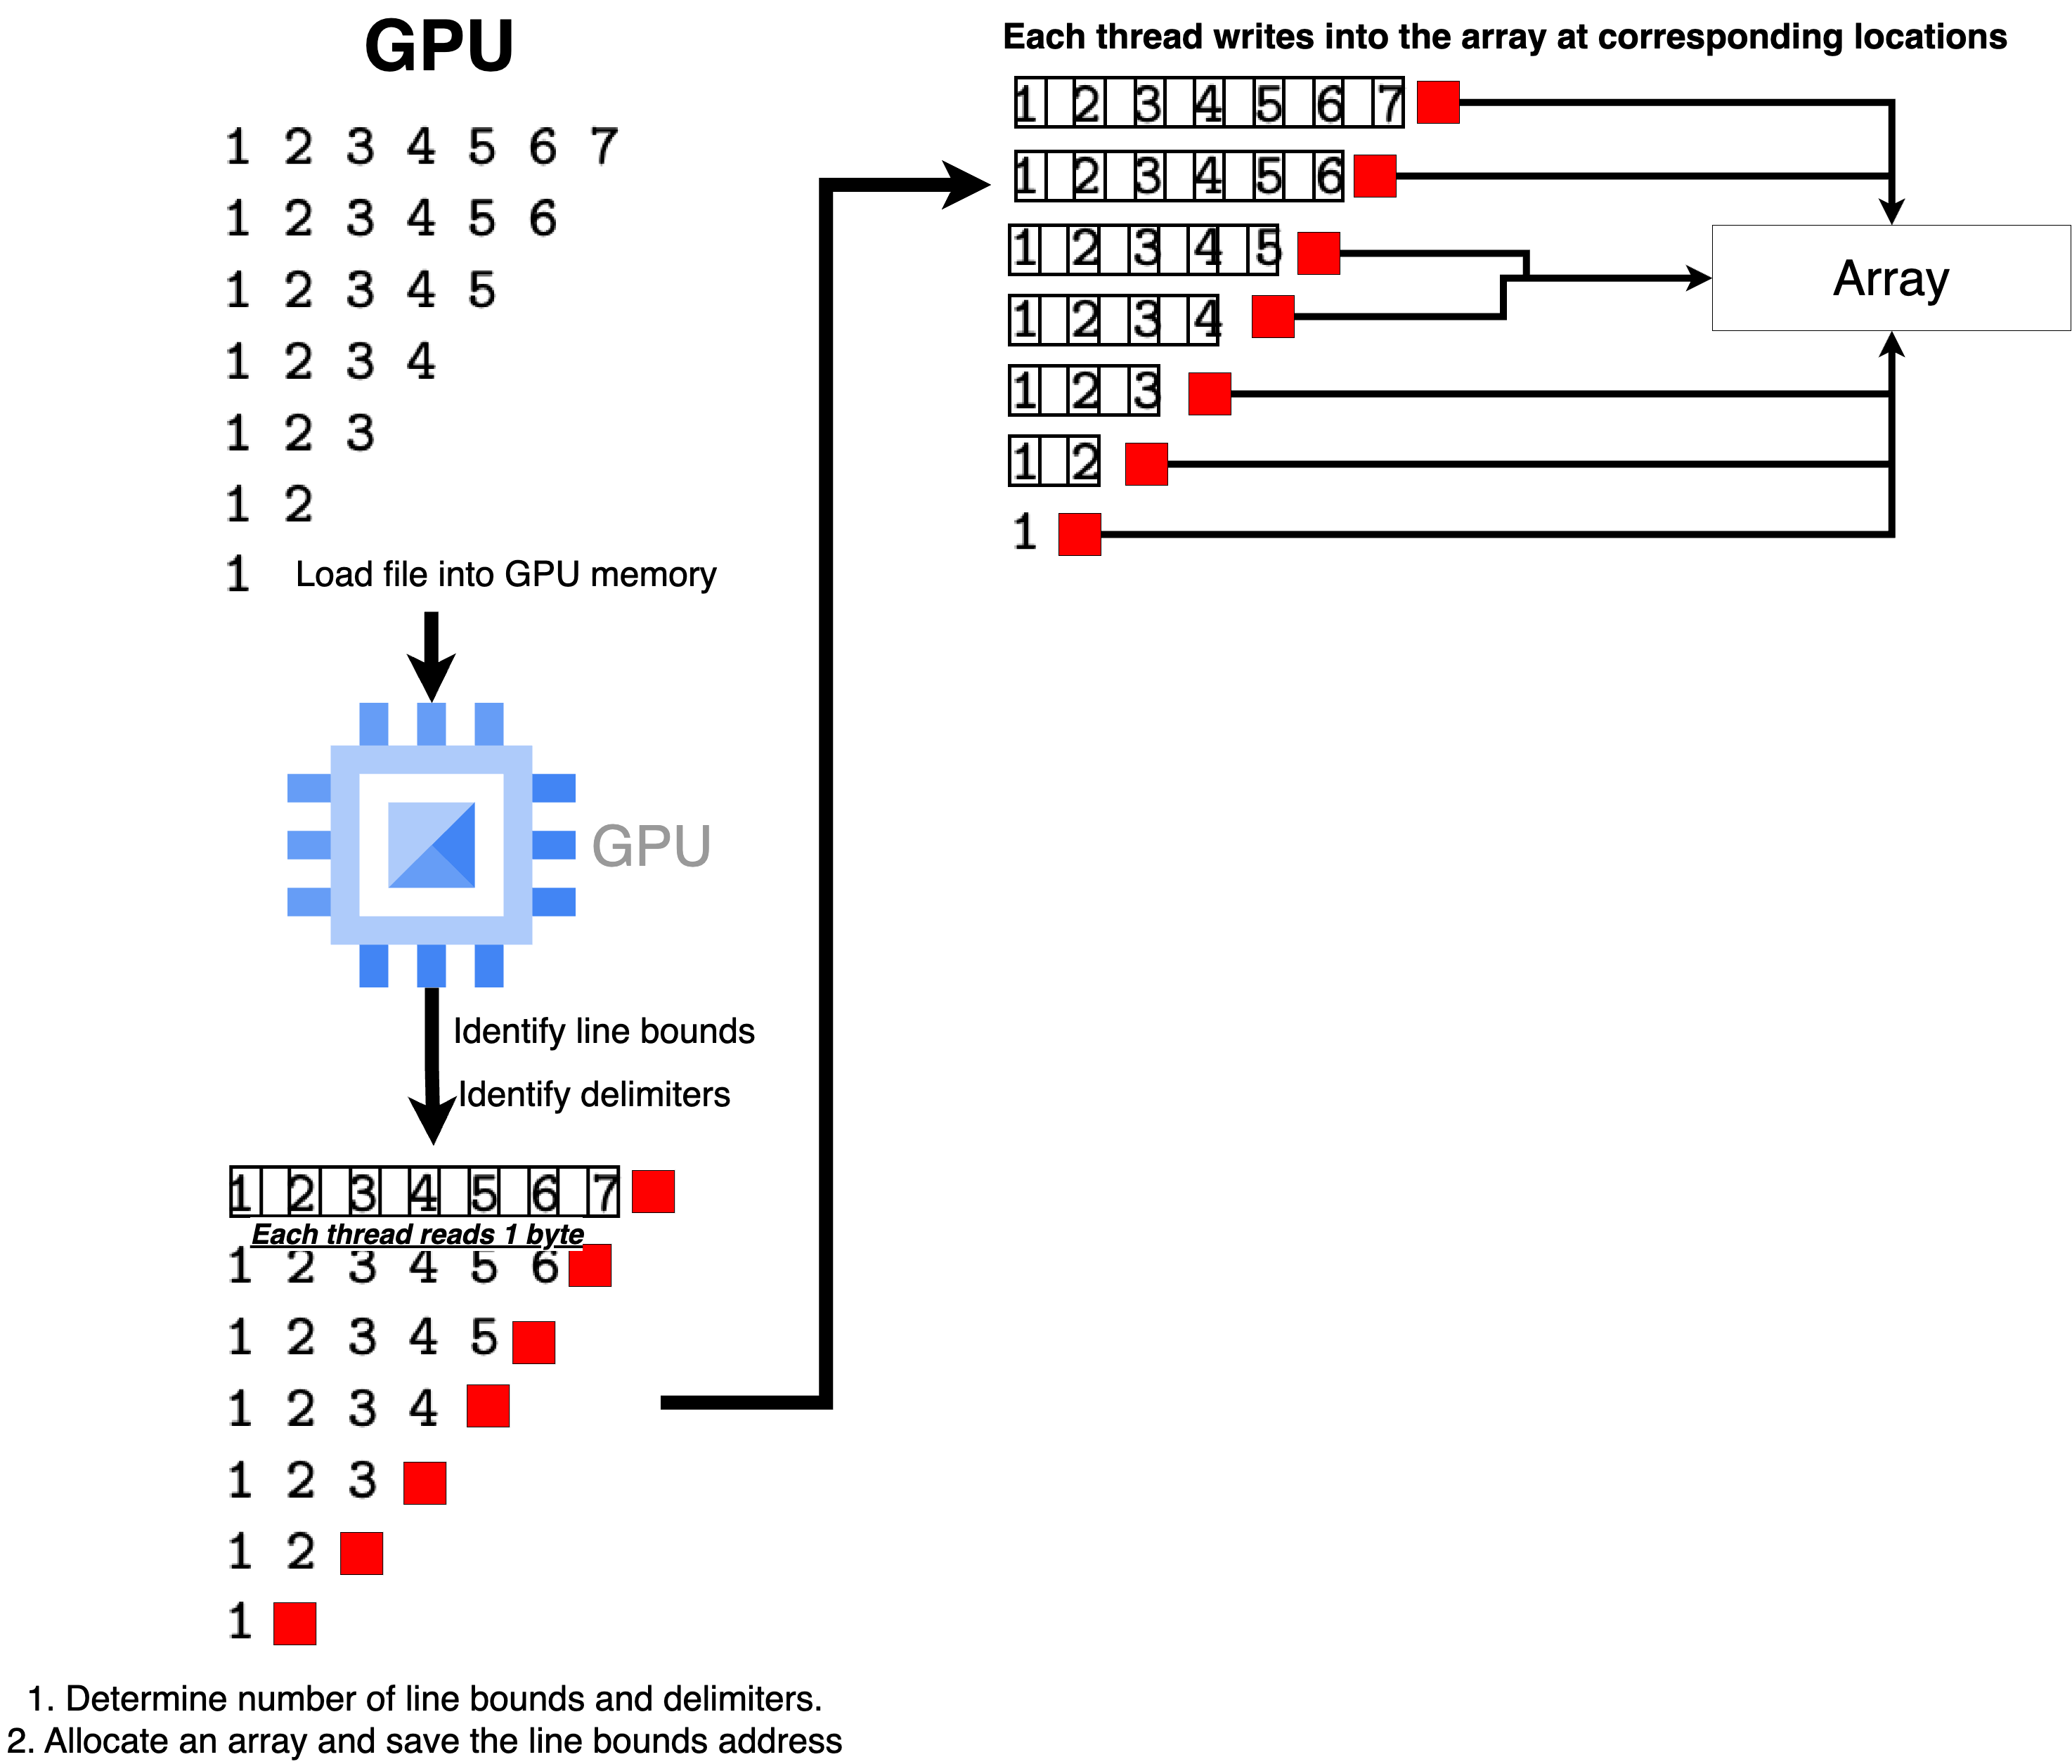
\includegraphics[width=0.8\textwidth]{2.png}
    \caption{GPU Read Process}
    \label{fig:gpu_read}
  \end{figure}
\end{frame}


\section{CPU Parser Method}
\begin{frame}{CPU Parser Approach}
  \begin{itemize}
    \item \textbf{Chunk Splitting:}
      \begin{itemize}
        \item The file is divided into equal-sized chunks.
      \end{itemize}
    \item \textbf{Boundary Adjustment:}
      \begin{itemize}
        \item Adjust the starting and ending points of each chunk to ensure that no chunk contains partial (incomplete) lines.
      \end{itemize}
    \item \textbf{Parallel Execution:}
      \begin{itemize}
        \item The number of chunks is determined by the number of available CPU cores.
        \item Each core processes one complete chunk concurrently, parsing the full lines in that segment.
      \end{itemize}
  \end{itemize}
\end{frame}

\begin{frame}{CPU Read Illustrated}
  \begin{figure}
    \centering
    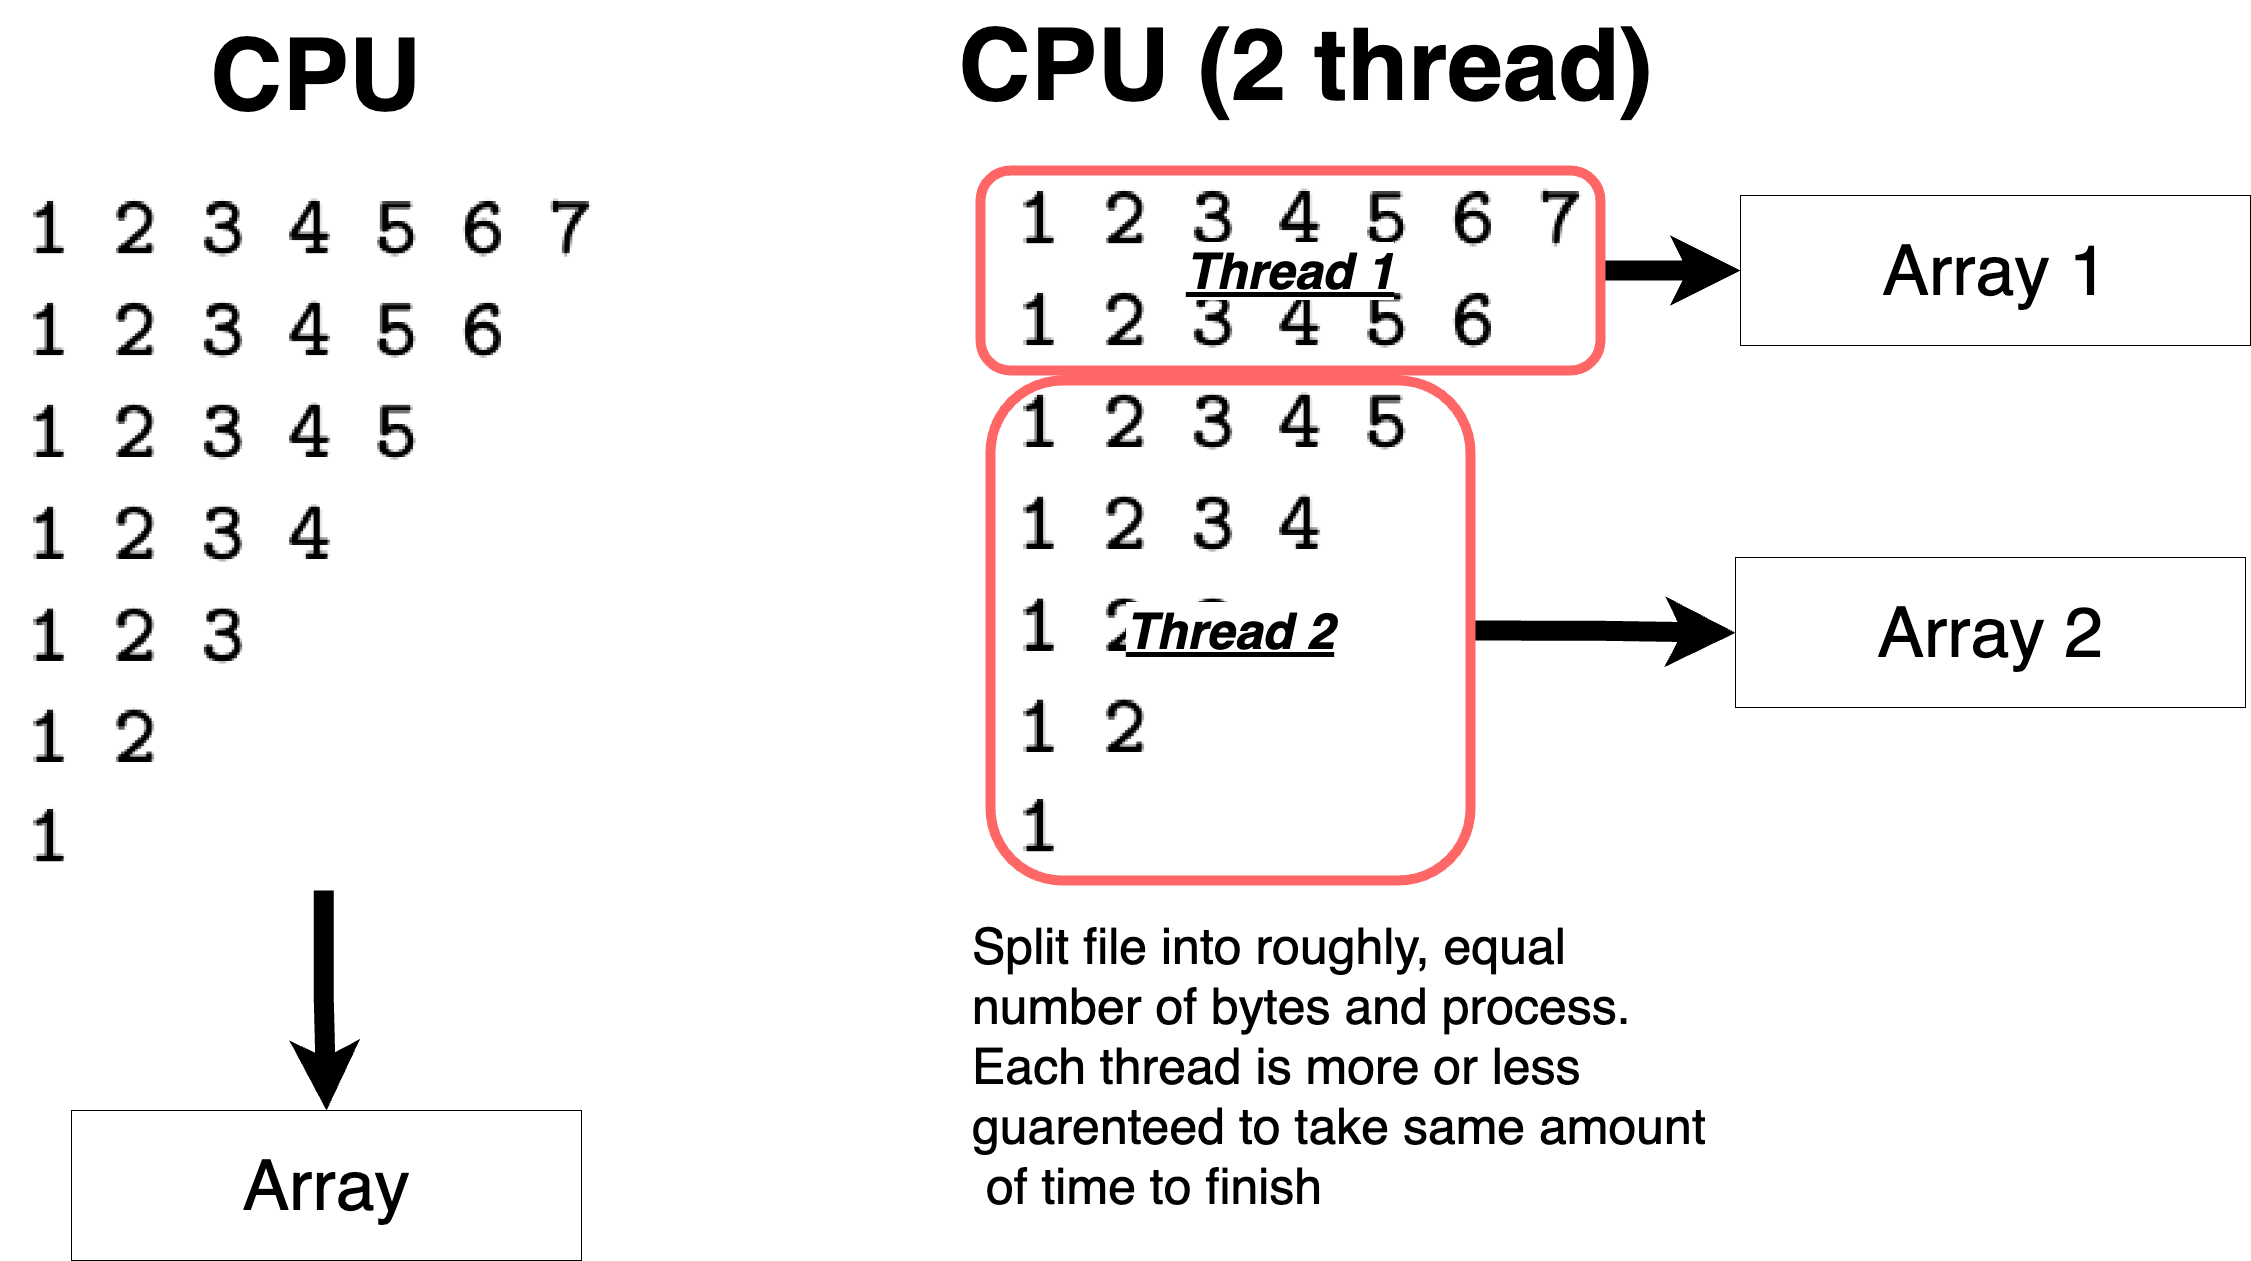
\includegraphics[width=0.8\textwidth]{1.png}
    \caption{CPU Read Process}
    \label{fig:cpu_read}
  \end{figure}
\end{frame}


% cuDF CSV Parser Slide
\section{cuDF CSV Parser}
\begin{frame}{cuDF CSV Parser}
  \begin{itemize}
    \item \textbf{Integration:} Part of the RAPIDS ecosystem, designed to work seamlessly with other GPU-accelerated libraries.
    \item \textbf{Performance:} Leverages GPU cores to achieve significant speed-ups compared to many CPU-based CSV parsers.
    \item \textbf{Ease of Use:} Simple integration with Python and familiar DataFrame interfaces.
  \end{itemize}
\end{frame}

\section{Experimental Setup}
\begin{frame}{Experimental Setup}

\begin{itemize}
  \item \textbf{Datasets:} Synthetic datasets with varying line sizes.
  \item \textbf{Hardware:} AMD Ryzen 5700X3D CPU, NVIDIA RTX 3070 GPU, 32GB RAM, and 256GB SSD (Max Read 400MB/s)
  \item \textbf{Software:} cuDF, cuPy, CPU and GPU parser implementations.
  \item \textbf{Methodology:}
    \begin{itemize}
      \item Load the datasets using custom GPU parser, cuDF CSV parser, and CPU methods.
      \item Measure execution time and resource utilization.
    \end{itemize}
\end{itemize}

\end{frame}

\begin{frame}
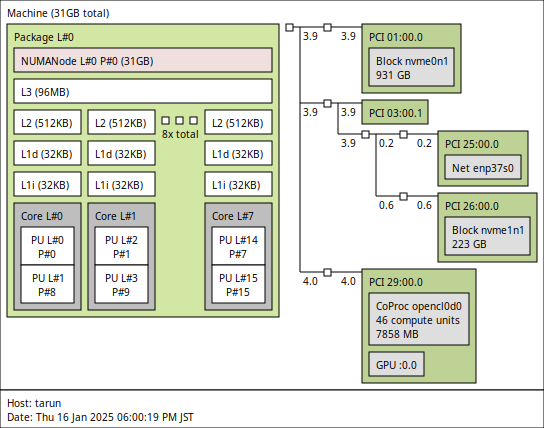
\includegraphics[width=0.9\textwidth]{topo.png}
\end{frame}

\begin{frame}
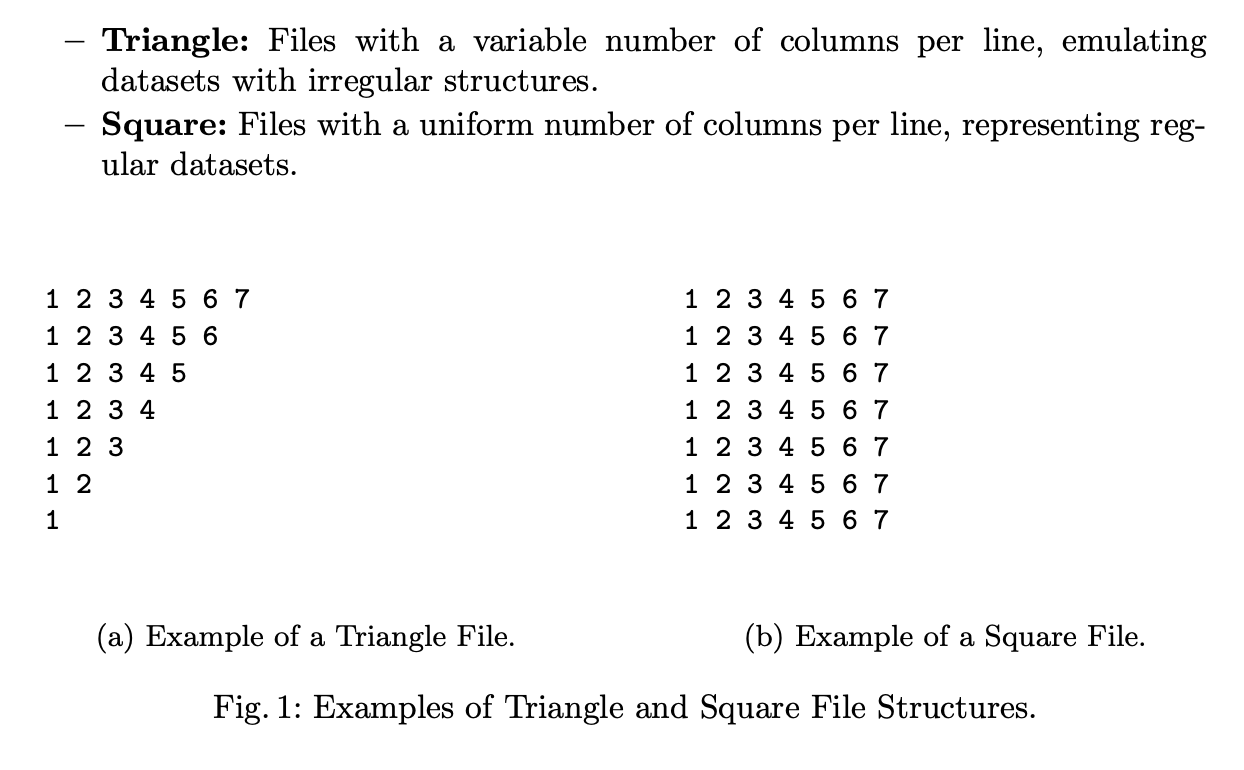
\includegraphics[width=0.9\textwidth]{image.png}
\end{frame}



% Experimental Results Slide
\section{Experimental Results}
\begin{frame}{Experimental Results}
  \begin{itemize}
    \item \textbf{Benchmark Setup:} Parsing large-scale datasets using both methods.
    \item \textbf{Metrics:} 
      \begin{itemize}
        \item Execution Time
        \item Resource utilization (GPU vs CPU).
      \end{itemize}
    \item \textbf{Preliminary Findings:}
      \begin{itemize}
        \item Both the custom GPU parser and cuDF CSV parser show similar speeds as CPU-based parser. SSD is the limiting factor.
        \item The custom GPU parser can be more finely optimized for specific data formats (e.g., non-integers) using asynchronous I/O and buffered reads for reduced memory usage.
      \end{itemize}
  \end{itemize}

  % % Optional: Insert a sample benchmark graph or table
  % \begin{figure}[h!]
  %   \centering
  %   \begin{subfigure}[b]{0.45\linewidth}
  %     \centering
  %     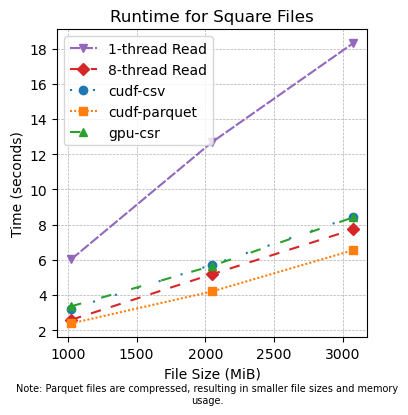
\includegraphics[width=\linewidth]{time_square.png}
  %     \caption{Execution Time: Square Data}
  %     \label{fig:time_square}
  %   \end{subfigure}
  %   \hfill
  %   \begin{subfigure}[b]{0.45\linewidth}
  %     \centering
  %     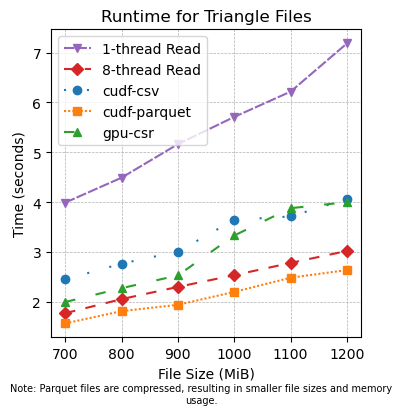
\includegraphics[width=\linewidth]{time_triangle.png}
  %     \caption{Execution Time: Triangle Data}
  %     \label{fig:time_triangle}
  %   \end{subfigure}
    
  %   \begin{subfigure}[b]{0.45\linewidth}
  %     \centering
  %     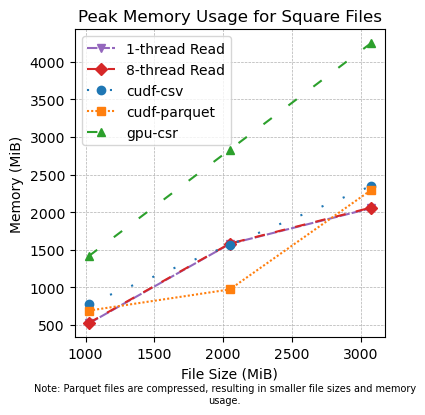
\includegraphics[width=\linewidth]{memory_square.png}
  %     \caption{Memory Usage: Square Data}
  %     \label{fig:memory_square}
  %   \end{subfigure}
  %   \hfill
  %   \begin{subfigure}[b]{0.45\linewidth}
  %     \centering
  %     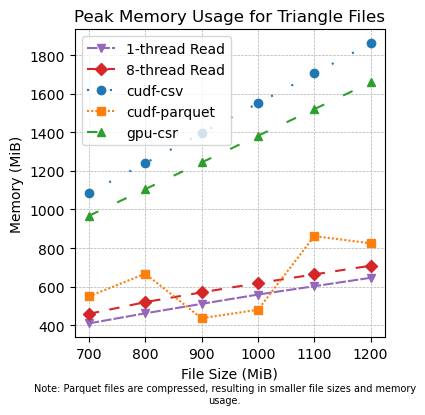
\includegraphics[width=\linewidth]{memory_triangle.png}
  %     \caption{Memory Usage: Triangle Data}
  %     \label{fig:memory_triangle}
  %   \end{subfigure}
    
  %   \caption{Benchmark Comparison of Execution Time and Memory Usage}
  %   \label{fig:benchmark_comparison}
  % \end{figure}

\end{frame}

\begin{frame}{Experimental Results}
 % Optional: Insert a sample benchmark graph or table
 \begin{figure}[h!]
  \centering
  \begin{subfigure}[b]{0.45\linewidth}
    \centering
    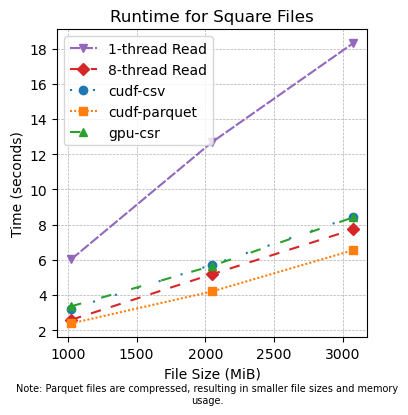
\includegraphics[width=\linewidth]{time_square.png}
    \caption{Execution Time: Square Data}
    \label{fig:time_square}
  \end{subfigure}
  \hfill
  \begin{subfigure}[b]{0.45\linewidth}
    \centering
    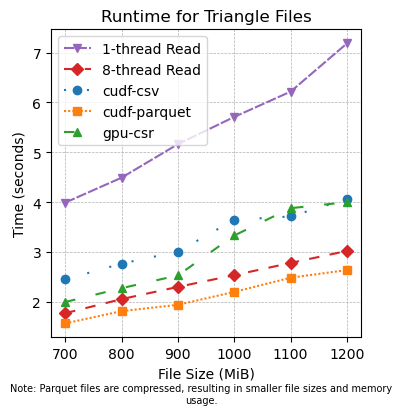
\includegraphics[width=\linewidth]{time_triangle.png}
    \caption{Execution Time: Triangle Data}
    \label{fig:time_triangle}
  \end{subfigure}
  
  % \begin{subfigure}[b]{0.45\linewidth}
  %   \centering
  %   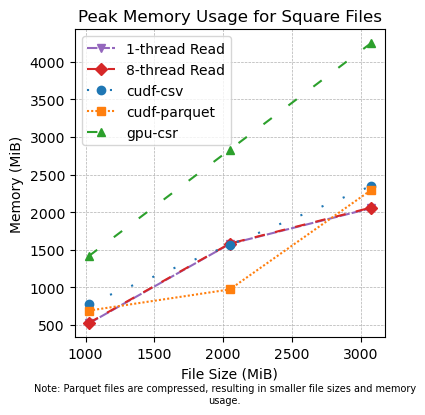
\includegraphics[width=\linewidth]{memory_square.png}
  %   \caption{Memory Usage: Square Data}
  %   \label{fig:memory_square}
  % \end{subfigure}
  % \hfill
  % \begin{subfigure}[b]{0.45\linewidth}
  %   \centering
  %   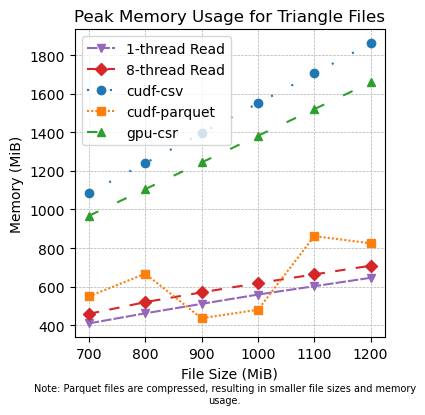
\includegraphics[width=\linewidth]{memory_triangle.png}
  %   \caption{Memory Usage: Triangle Data}
  %   \label{fig:memory_triangle}
  % \end{subfigure}
  
  \caption{Benchmark Comparison of Execution Time and Memory Usage}
  \label{fig:benchmark_comparison}
\end{figure}

\end{frame}

\begin{frame}{Experimental Results}
  % Optional: Insert a sample benchmark graph or table
  \begin{figure}[h!]
   \centering
  %  \begin{subfigure}[b]{0.45\linewidth}
  %    \centering
  %    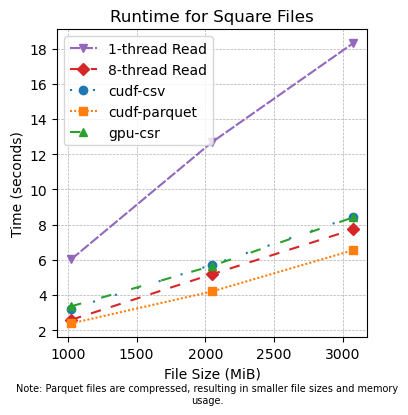
\includegraphics[width=\linewidth]{time_square.png}
  %    \caption{Execution Time: Square Data}
  %    \label{fig:time_square}
  %  \end{subfigure}
  %  \hfill
  %  \begin{subfigure}[b]{0.45\linewidth}
  %    \centering
  %    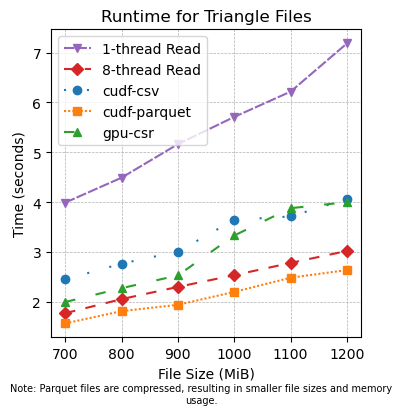
\includegraphics[width=\linewidth]{time_triangle.png}
  %    \caption{Execution Time: Triangle Data}
  %    \label{fig:time_triangle}
  %  \end{subfigure}
   
   \begin{subfigure}[b]{0.45\linewidth}
     \centering
     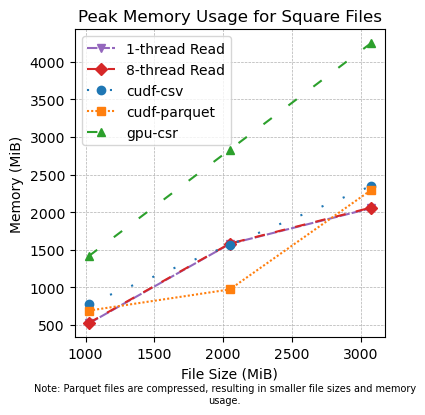
\includegraphics[width=\linewidth]{memory_square.png}
     \caption{Memory Usage: Square Data}
     \label{fig:memory_square}
   \end{subfigure}
   \hfill
   \begin{subfigure}[b]{0.45\linewidth}
     \centering
     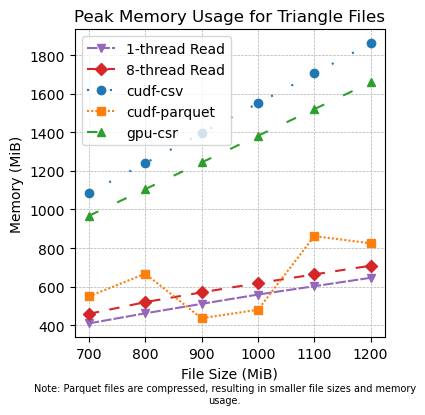
\includegraphics[width=\linewidth]{memory_triangle.png}
     \caption{Memory Usage: Triangle Data}
     \label{fig:memory_triangle}
   \end{subfigure}
   
   \caption{Benchmark Comparison of Execution Time and Memory Usage}
   \label{fig:benchmark_comparison}
 \end{figure}
 
 \end{frame}


% % Conclusion Slide
% \section{Conclusion}
% \begin{frame}{Conclusion}
%   \begin{itemize}
%     \item GPU-based methods can provide substantial performance improvements in data parsing tasks.
%     \item The choice between a custom GPU parser and cuDF's built-in CSV parser depends on factors such as customization needs, available resources, and integration with existing workflows.
%     \item For Parquet file formats, cuDF offers an excellent GPU-accelerated alternative to traditional CPU methods.
%     \item Future work is to explore this experiment on larger datasets with larger GPU memory.
%     \item Incoporate BaM's work to extend available GPU memory and optimize/port the custom GPU parser to the BaM platform.
%   \end{itemize}
% \end{frame}

% % Questions Slide
% \begin{frame}{Questions}
%   \centering
%   {\Large Any Questions?}
% \end{frame}

\end{document}
